\chapter{System Engineering and Design}  
\label{chap3}  

% ====== Section 1: Requirements ======  
\section{System Requirements} 
{ 
The system is designed for low-cost, real-time vibration monitoring of rotating machinery. This set-up encompasses components that are of major importance and its aim is to collect data within a specific - prerequired range, store data safely at a database and finally process data.

The following sections include more detailed overview of the system requirements. Hereunder, more details will be elaborated.
}

\subsection{Functional Requirements} 
{ 
The most commonly rotating speed of machinery goes up to 1500 [rpm] corresponds to 25 [Hz]. This relationship is defined by the following equation: 

\begin{equation}
	f \, [\mathrm{Hz}] = \frac{r \, [\mathrm{RPM}]}{60}
\end{equation}

The aforementioned relationship entails that the rotational speed of a machine can be interpreted in frequency, which in turn is of great help when related to Fourier Transform applications.

All in all, the functional requirements are highlighted hereunder:
\begin{itemize}  
	\item \textbf{Frequency Range}: 0–300 Hz (covers common machine faults like imbalance, misalignment).  
	\item \textbf{Real-Time Processing}: On-the-fly FFT computation for immediate fault detection.  
	\item \textbf{Scalability}: Modular design for multi-sensor deployments.  
\end{itemize}  
}

\subsection{Non-Functional Requirements} 
{ 
\begin{itemize}  
	\item \textbf{Cost}: Minimize BOM cost (justifies Arduino + RPi4 over industrial PLCs).  
	\item \textbf{Power}: Optimize for continuous operation (e.g., no active cooling).  
	\item \textbf{Accuracy}: ADXL335’s ±3g range suffices for industrial vibrations (cite datasheet).  
\end{itemize}  
}

% ====== Section 2: Hardware Design ======  
\section{Hardware Architecture}  
\subsection{Component Selection}  
{
\begin{itemize}  
	\item \textbf{ADXL335 Accelerometer}:  
	\begin{itemize}  
		\item Analog output simplifies Arduino ADC interfacing.  
		\item 300Hz bandwidth meets requirements (vs. digital sensors like MPU6050 needing I2C).  
	\end{itemize}  
	\item \textbf{Arduino Uno}:  
	\begin{itemize}  
		\item Handles analog sampling at 600Hz (Nyquist-compliant for 300Hz signals).  
		\item Low-latency preprocessing (e.g., DC removal, windowing).  
	\end{itemize}  
	\item \textbf{Raspberry Pi 4}:  
	\begin{itemize}  
		\item Runs Python-based FFT (e.g., NumPy) and SQLite for local storage.  
		\item WiFi/Bluetooth enables cloud integration (e.g., AWS IoT, InfluxDB).  
	\end{itemize}  
\end{itemize}  

\begin{figure}[h]  
	\centering  
	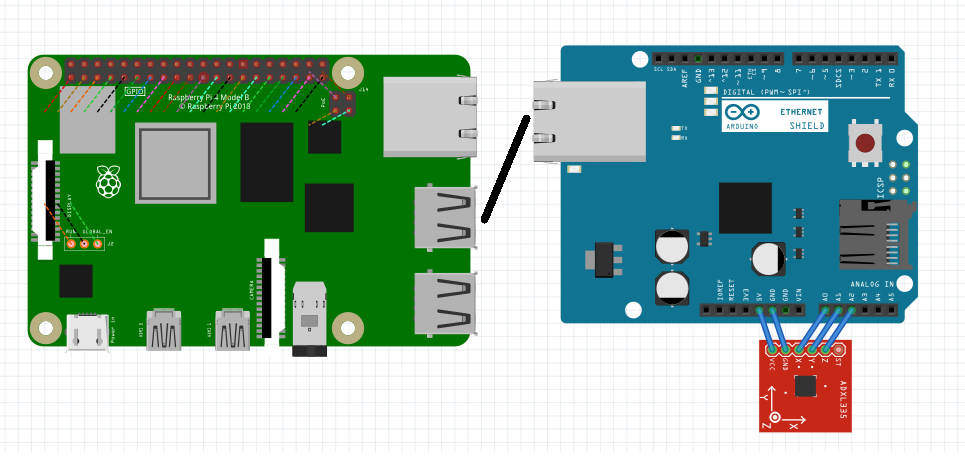
\includegraphics[width=\linewidth]{figures/System.png}  
	\caption{Hardware architecture with signal flow}  
	\label{fig:System}  
\end{figure}
}  

% ====== Section 3: Software & Data Flow ======  
\section{Software Architecture and Data Flow}
 
\subsection{Signal Processing Pipeline} 
{
The Arduino samples data at 600Hz, which is extremely high and constitutes a sufficient sample rate for this project. Additionally, another consideration is receiving data from the ADXL335 sensor breakout, which could potentially make this procedure slower. The highest data volume over a predefined time span achieved for this project is 300Hz.

In essence, a batch of data is received through this procedure by a Raspberry Pi 4, which in turn processes and analyzes these samples.
}  

\subsection{Scalability Considerations}
{  
\begin{itemize}  
	\item \textbf{Multi-Threading}: RPi4 handles concurrent sensor inputs (e.g., 4x Arduino nodes).  
	\item \textbf{Data Compression}: FFT bin reduction (0–300Hz only) minimizes cloud costs.  
\end{itemize}  

\begin{figure}[h]  
	\centering  
	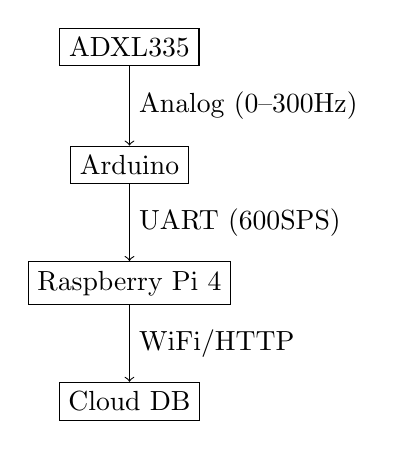
\begin{tikzpicture}[node distance=1.5cm]  
		\node (sensor) [draw, rectangle] {ADXL335};  
		\node (arduino) [draw, rectangle, below of=sensor] {Arduino};  
		\node (rpi) [draw, rectangle, below of=arduino] {Raspberry Pi 4};  
		\node (cloud) [draw, rectangle, below of=rpi] {Cloud DB};  
		
		\draw[->] (sensor) -- node[right] {Analog (0–300Hz)} (arduino);  
		\draw[->] (arduino) -- node[right] {UART (600SPS)} (rpi);  
		\draw[->] (rpi) -- node[right] {WiFi/HTTP} (cloud);  
	\end{tikzpicture}  
	\caption{End-to-end data flow with protocols}  
	\label{fig:Flowchart}  
\end{figure}  
}

\subsection{Arduino sketch}
{
Elaboration on (including the whole code):
\begin{itemize}
\item Description of sketch and cpp files
\item elaborate on how it shares data via UART
\item Analyse the possibility of translating Voltage into g or m/s2
\end{itemize}
}

\subsection{Raspberry Pi coding}
{
Elaboration on (including some parts of the code):
\begin{itemize}
\item Description of the whole program
\item how it posts data via HTTP
\item Data stored on database , and database setup
\end{itemize}
}

\subsection{Vercel coding}
{
Elaboration on (including some parts of the code):
\begin{itemize}
\item page file that prints data
\item how it is coupled with supabase
\end{itemize}
}
